%
%%%%%%%%%%%%%%%%%%%%%%%%%%%%%%%%%%%%%%%%%%%%%%%%%%%%%%%%%%
%
%  U M S E T Z U N G   &   I M P L E M E N T I E R U N G
%
%%%%%%%%%%%%%%%%%%%%%%%%%%%%%%%%%%%%%%%%%%%%%%%%%%%%%%%%%%
\chapter{Umsetzung \& Imlementierung}
\label{cha:umsetzung}
%
Nun kommen wir an den praktischen Teil der Arbeit. In diesem Kapitel wird zunächst einiges über die Entwicklungsumgebung gesagt. Anschließend wird auf wesentliche Punkte der Umsetzung und Implementierung eingegangen. Dabei wird wieder auf die Anforderungen zurückgegriffen und erläutert wie diese umgesetzt wurden. Vorraussetzung für dieses Kapitel ist das Grundlagenkaptitel der Arbeit, um zusammenhänge mit den Technologien besser verstehen zu können.
\section{Entwicklungsumgebung}
\label{sec:umsetzung}
%
Dieses Kapitel befasst sich mit den verwendeten Technologien, die eine produktive Entwicklung ermöglichen. Es wird auf alle verwendeten Technologien, Bibliotheken sowie Programme eingegangen und begründet, warum eine Verwendung sinnvoll ist.\\
\paragraph{Technologien und Bibloetheken}
Wie in den vergangenen Kapiteln schon erläutert sind die Haupttechnologien das Framework \textit{Angular} sowie die 3D Bibliothek \textit{Three.js}, welche WebGL zum Einsatz bringt. Angular Anwendungen werden grundsätzlich mit \textit{Node.js} installiert. Dadurch ist es uns später möglich verschiedene npm-Module wie Three.js oder auch Bootstrap zu installieren. Zusätzlich nutzt Angular \textit{Webpack}, um den Quellcode zu bündeln. Dabei werden die scss-Dateien in eine css-Datei komprimiert. Sass in Verbindung mit \textit{Webpack} ist nicht nur in für Angular-Projekte ein beliebtes Tool zum entwickeln von Webseiten und Webanwendungen. Auch eine Versionierung des Quellcodes kommt zum Einsatz. Mit \textit{Git} ist der Quellcode immer gesichert und man kann nach dem Testen einer bestimmten Funktion immer wieder zum letzten Push zurückkehren. Bei einem Bachlor-Projekt kann man zwar nicht den Vorteil der Teamentwicklung mit \textit{Git} nutzen, jedoch kann man damit sehrwohl seinen Quellcode versionieren und sichern, was bei einem Bachlorprojekt durchaus sinnvoll erscheint. 
\paragraph{Entwicklungswerkzeuge} Als Text-Editor wird \textit{PhpStorm} verwendet. Dadurch ist eine flexible Programmierung an unterschiedlichen Systemen möglich, da der Editor für Windows, MacOS als auch für Linux verfügbar ist. Er bietet eine praktische Integration von Git und kann dazu noch sehr gut mit Angular-Anwendungen arbeiten. Auch Angular CLI Befehle können teilweise direkt in dem Editor ausgeführt werden und \textit{PhpStorm} verfügt über eine logische Code-Verfolständigung. Nicht zu vergessen die optimale Quellcode-Formatierung für jeden Dateityp. \textit{PhpStorm} verfügt zwar über ein integriertes Terminal, jedoch ist das meist sehr unpraktisch, da es nur unnötig Platz in der Anwendung wegnimmt. Deswegen werden Kommandozeilen einem zusätzlichen Terminal ausgeführt. Gerade am Anfang des Projekts wird die Angular CLI viel zum Einsatz kommen.
%
\section{Anlegen des Angular-Projekts}
\label{sec:umsetzung}
%
Bevor die Angular-Anwendung nach und nach aufgebaut werden kann, muss Angular erst einmal installiert werden und anschließend ein Projekt erstellt werden. Mit der Angular CLI ist das sehr einfach und unproblematisch. Deshalb ist der erste Schritt diese über Node.js zu installieren.
%
\section{Module des Konfigurators}
\label{sec:umsetzung}
%
Im folgenden Kapitel wird betrachtet aus welchen Module die Angular Anwendung aufgebaut ist. Anschließend werden die Module angelegt. Es geht hier nur um das Anlegen der Module, noch nicht um die Funktionalität der einzelnen Module. Die Abbildung zeigt eine Übersicht aller Module, welche in der Webanwendung implementiert sind\footnote{Hierbei ist zu beachten, dass die Abbildung auf die wesentlichen Module beschränkt ist, da es sonst zu unübersichtlich werden würde. Eine vollständige Übersicht der Module befindet sich im Anhang.}.
\begin{figure}[h]
	\centering
	{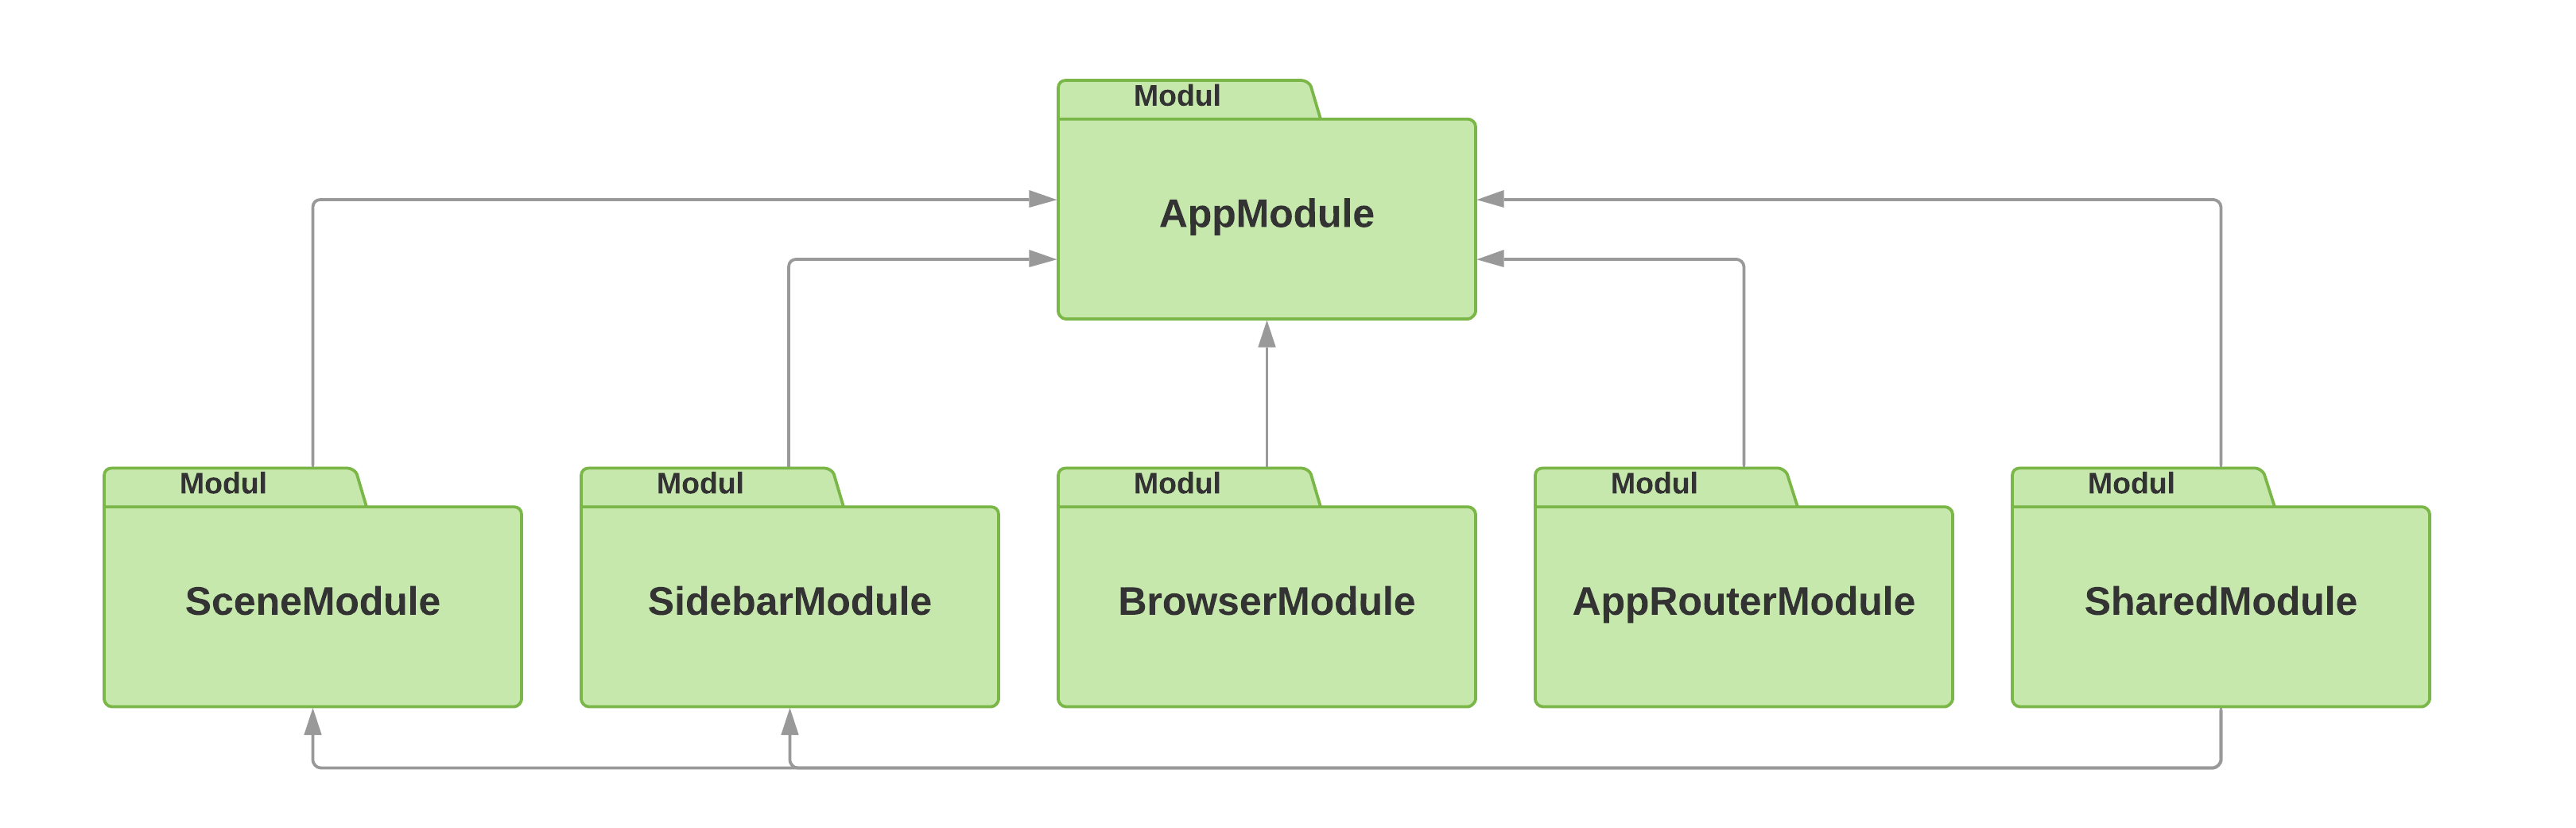
\epsfig{file = umsetzung/images/module.png, width=13.0cm}}
	\caption[Komponentendiagramm]{\textit{Module der Angular-Anwendung}}
	\label{fig:module}
\end{figure}
Die einzelnen Bausteine der Angular-Anwendung werden im Rahmen dieses Bachlorprojektes immer über die Angular CLI generiert, da das am einfachsten funktioniert und zeitsparend ist. Ein Modul kann mit folgendem Command Line Befehl generiert werden:
%
\begin{lstlisting}
ng g m shared
\end{lstlisting}
%
Als Beispiel wurde hier das Module \textit{shared} angelegt. Hierin werden später alle globalen Bausteine der Angular-Anwendung erstellt. Es wurden außerdem die Appkürzungen \texttt{m} für \texttt{module} und \texttt{g} für \texttt{generate} verwendet. Ob ausgeschrieben oder abgekürzt, das hat keine Auswirkungen, sondern spart lediglich Zeit. Es gibt noch ein paar Zusatzoptionen, die als Parameter angegben werden können. Diese sind in der offizielen Dokumentation von Angular aufgeführt. Diese ermöglichen verschiedene Funktionen wie \texttt{export}-Funktion oder verhindern das generieren von Testdateien. Der 3D Konfigurator hat noch zwei weitere wichtige Module. Zum einen ist das \textit{SceneModule} für die 3D Darstellung zuständig und das Rendern des Designs. Das \textit{SidebarModule} ist sozusagen das Konfigurationsmenu inklusive einer Übersicht in tabellarischer Form. Die hauseigenen Module von Angular wie das \textit{BrowserModule} wurden von der Angular CLI automatisch importiert. Hier ist also kein weiterer Schritt notwendig, die Anwendung sollte lauffährig sein. Noch hat die Applikation allerdings noch keine richtige Funktionalität.
%
\section{Komponenten des Konfigurators}
\label{sec:umsetzung}
%
Sowohl das \textit{SidebarModule} als auch das \textit{SceneModulue} des Konfigurators haben sozusagen eine \glqq Hauptkomponente\grqq. Diese werden dann später in der \textit{AppComponent} eingebunden. Die Basis-Komponente der Anwendung ist also sehr einfach und übersichtlich. Dann gibt es noch einige weitere Kindskomponenten sowie geteilte Komponenten (aus dem \textit{sharedModule}). In diesem Kapitel werden wir uns zunächst auf die Komponenten beschränken. Alle weiteren Bausteine wie Services werden wir später noch genauer betrachten.\\
Die \textit{SceneComponent} ist dafür da die komplette 3D-Szene zu erzeugen und eben das Becher-Model mit seinem Design darstellen soll. Wie alle Kompoentente wurde diese mittels Angular CLI in PhpStorm angelegt, wie in Abbildung \ref{fig:phpstorm} zu sehen. 
%
\begin{figure}[h]
	\centering
	\subfigure[Auswahl generierbarer Angular-Bausteine]{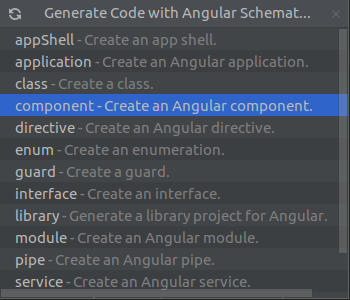
\includegraphics[width=5cm\textwidth]{umsetzung/images/auswahlcli.png}}
	\subfigure[Gernerieren einer Komponente mit Parametern]{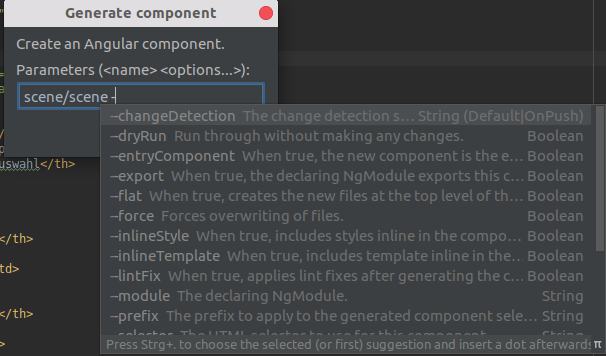
\includegraphics[width=7cm\textwidth]{umsetzung/images/optionscli.png}}\\
	\subfigure[Generierte Dateien durch die CLI]{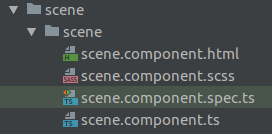
\includegraphics[width=5cm\textwidth]{umsetzung/images/generatedfiles.png}}
	\caption{\textit{Erstellung einer Angular-Komponente mit PhpStorm}}
	\label{fig:phpstorm}
\end{figure}
%
In PhpStorm kann man über \lstinline{File > New > Angular Schematics} innerhalb des Editors die Angular CLI verwenden. Wie im ersten Bild zu sehen, lassen sich so alle Bausteine von Angular anlegen. In diesem Fall wird eine Komponente angelegt. Nach der Auswahl wird man nun aufgefordert den Komponenten-Namen sowie optionale Parameter mit anzugeben. Das praktische ist, das PhpStorm alle verfügbaren Parameter vorschlägt und man nicht etwa in der Documentation nachschauen müsste, welchen Parameter man braucht und vermeidet Tippfehler. Nach bestätigen der Eingabe werden nun wie in Bild c) zu sehen alle erforderlichen Dateien der Komponente generiert. Zusätzlich werden im Hintergrund eventuelle Import-Anweisungen sowie Export- Anweisungen und so weiter automatisch ergänzt. In unserem Fall wurden auch die Testdatei erzeugt, welche wir uns im nächsten Kapitel genauer anschauen wollen. Die anderen drei Dateien sind wie wir wissen für Logik, Styles und Templating zuständig. Analog zu dem Erstellen der Komponente in PhpStorm funktioniert das ganze auch in einem Terminal:
%
\begin{lstlisting}
ng g c scene/scene -m=scene
\end{lstlisting}
%
Sobald die Komponente angelegt ist, hat sich eigentliche keine Funktionalität. Das wird erst später mit der Logik und den Services implementiert. Für den Anfang reicht es, hier schonmal das \texttt{canvas}-Element anzulegen und ein paar Styles in der \texttt{scss}-Datei der Komponente anzulegen. Wer sich mit \texttt{scss} bzw. \texttt{sass} auskennt, kann hier die Schreibweise nutzen. Man kann aber auch normales \texttt{css} schreiben. Damit ist die \textit{SceneComponent} im Grunde schon fertig.
\paragraph{Kindskomponente}
Genauso \textit{SceneComponent} wurde auch die \textit{SidebarComponent} angelegt. Sie stellt die komplette Sidebar im rechten Bereich dar, also das Konfigurationsmenü und die Übersicht. Diese Komponente hat noch ein paar Kindskomponenten. Die Sidebar ist mit der Bootstrap-Komponente \textit{Tabs}\footnote{https://getbootstrap.com/docs/4.0/components/navs/\#tabs} umgesetzt. Wir haben also im Menu zwei Tabs, Konfigurator und Übersicht. Diese Tabs sind als eigene Komponente in \textit{SharedModule} implementiert und können in unserer SidebarCompontent also KindsKomponente verwendet werden. Die Umsetzung der Tab-Komponente wird nun genauer beleuchtet.\\
Die Tabs von Bootstrap sind als \texttt{<ul>}-Element implementiert. Die einzelnen Tabs sind also die \texttt{<li>}-Elemente und werden in der unordered-List gebündelt. Am Ende entsteht folgendes Template für die Tabs-Komponente:
%
\begin{lstlisting}
<ul class="nav nav-tabs nav-fill">
	<li class="nav-item" *ngFor="let tab of tabs" (click)="selectTab(tab)">
		<a [class.active]="tab.active" class="nav-link nav-title" href="#"><span class="mr-3 mdi mdi-gauge"></span>{{tab.title}}</a>
	</li>
</ul>
<ng-content></ng-content>
\end{lstlisting}
%
Die ul-Liste ist eigentlich identisch zur normalen Syntax. Dieser stellt den Container für die einzelnen Tabs da. Um das ganze dynamisch umzusetzten sollte die Komponente eine beliebige Anzahl an Tabs haben können. Deshalb sind die li-Tags hier mit einer Direktive von Angular verkünpft: mit ngFor werden in einer Schleife alle Tab-Title erstellt. Bei onclick soll bekanntlich der Tab als aktiv makiert werden und dessen Content angezeigt werden. Das regelt die SelectTab() Methode. Sie sagt der Kompoenente welchen inhalt sie nun anzeigen soll.
- Tabs als ul liste li einzelner Tab
- einzelner Tab extra klasse (Template zeigen)
- Einzelne Tab Variable für Titel und Activ-Status
-TabsComponent nutzt Tab und bekommt von ihr die inputs



Zusätzlch hat die SidebarComponent auch noch eigene nicht geteilte Kindskompontenten. Das Konfigurationsmenü besteht aus Größe, Design-Upload und Optionen. Diese drei sind ebenfalls als Menü umgesetzt. Es handelt sich hier wieder um eine Bootstrap Komponente, das Accordeon. Die einzelnen Punkte sind hier auch wieder eigenständige Komponenten die als KindsKomponenten in sidebarComponent verwendet werden.
Diese Vorlage verwendet die \textit{memoir}-LaTeX-Klasse von Peter Wilson und erzeugt somit ein Buchdokument, das auch zweiseitig gedruckt werden sollte, da zwischen den Kapiteln Leerseiten erzeugt werden. Einstiegspunkt für die Bachelorarbeit ist die Datei \texttt{abschlussarbeit.tex}. Tragen Sie zunächst den Titel der Arbeit und alle Namen ein. Bei hochschulinternen Bachlorarbeiten fallen die Eintragungen \textit{durchgeführt am} und \textit{Betreuer in der Firma} natürlich weg.
%
\section{3D Szene mit Model}
\label{sec:umsetzung}
%
Diese Vorlage verwendet die \textit{memoir}-LaTeX-Klasse von Peter Wilson und erzeugt somit ein Buchdokument, das auch zweiseitig gedruckt werden sollte, da zwischen den Kapiteln Leerseiten erzeugt werden. Einstiegspunkt für die Bachelorarbeit ist die Datei \texttt{abschlussarbeit.tex}. Tragen Sie zunächst den Titel der Arbeit und alle Namen ein. Bei hochschulinternen Bachlorarbeiten fallen die Eintragungen \textit{durchgeführt am} und \textit{Betreuer in der Firma} natürlich weg.
\paragraph{3D-Szenen-Service}
\section{Design Rendering}
\label{sec:umsetzung}
%
Diese Vorlage verwendet die \textit{memoir}-LaTeX-Klasse von Peter Wilson und erzeugt somit ein Buchdokument, das auch zweiseitig gedruckt werden sollte, da zwischen den Kapiteln Leerseiten erzeugt werden. Einstiegspunkt für die Bachelorarbeit ist die Datei \texttt{abschlussarbeit.tex}. Tragen Sie zunächst den Titel der Arbeit und alle Namen ein. Bei hochschulinternen Bachlorarbeiten fallen die Eintragungen \textit{durchgeführt am} und \textit{Betreuer in der Firma} natürlich weg. 
\paragraph{3D Zylinder für Design rendering}
%https://threejs.org/docs/#api/en/geometries/CylinderBufferGeometry\\
%https://threejs.org/docs/#api/en/core/BufferGeometry\\
%https://codepen.io/JasonStoltz/pen/NaBOGm (transparente Designs) \\
%https://www.flyeralarm.com/sheets/de/becher_kstoff_200ml.pdf\\
%https://stackoverflow.com/questions/55283187/threejs-texture-fit-uv-map\\

\section{Mobile Sidebar}
\label{sec:umsetzung}
%
Das Off-Canvas Menu ist vom Design nicht anders als die Desktop Variante. Es wird lediglich verschoben. Es handelt sich dabei um eine JavaScript Funktion, die einfach das Menü aus dem sichtbaren Bereich verschiebt und sie erst dann sichtbar werden lässt, wenn der  Hamburger-Menu-Button gedrückt wird. Über Css werden die SceneComponent sowie die SidebarComponent noch als vollflächig dargestellt und schon ist das Mobile Menü fertig.
Diese Vorlage verwendet die \textit{memoir}-LaTeX-Klasse von Peter Wilson und erzeugt somit ein Buchdokument, das auch zweiseitig gedruckt werden sollte, da zwischen den Kapiteln Leerseiten erzeugt werden. Einstiegspunkt für die Bachelorarbeit ist die Datei \texttt{abschlussarbeit.tex}. Tragen Sie zunächst den Titel der Arbeit und alle Namen ein. Bei hochschulinternen Bachlorarbeiten fallen die Eintragungen \textit{durchgeführt am} und \textit{Betreuer in der Firma} natürlich weg.
%
\section{Daten-Service}
\label{sec:umsetzung}
%
Der DataService hat eine Aufgabe: Alle Daten des konfigurierten Bechers zu speichern und sie bei Anfrage einer Komponente wieder zurückzugeben. Dabei ist es wichtig das der Service nur einmal gestartet wird und die Daten global speichert. Hierbei handelt es sich also um ein Singelton.
Diese Vorlage verwendet die \textit{memoir}-LaTeX-Klasse von Peter Wilson und erzeugt somit ein Buchdokument, das auch zweiseitig gedruckt werden sollte, da zwischen den Kapiteln Leerseiten erzeugt werden. Einstiegspunkt für die Bachelorarbeit ist die Datei \texttt{abschlussarbeit.tex}. Tragen Sie zunächst den Titel der Arbeit und alle Namen ein. Bei hochschulinternen Bachlorarbeiten fallen die Eintragungen \textit{durchgeführt am} und \textit{Betreuer in der Firma} natürlich weg.
%
\section{Upload-Vorgang}
\label{sec:umsetzung}
%
Diese Vorlage verwendet die \textit{memoir}-LaTeX-Klasse von Peter Wilson und erzeugt somit ein Buchdokument, das auch zweiseitig gedruckt werden sollte, da zwischen den Kapiteln Leerseiten erzeugt werden. Einstiegspunkt für die Bachelorarbeit ist die Datei \texttt{abschlussarbeit.tex}. Tragen Sie zunächst den Titel der Arbeit und alle Namen ein. Bei hochschulinternen Bachlorarbeiten fallen die Eintragungen \textit{durchgeführt am} und \textit{Betreuer in der Firma} natürlich weg.